\documentclass[spanish]{udpreport}
\usepackage[utf8]{inputenc}
\usepackage[spanish]{babel}

% Podemos establecer el logo de alguna entidad o dejar el de la UDP (defecto)
%\setlogo{EITFI}

\title{Informe de redes de datos 3\\
"Creación de paquetes con Scapy y validación con Wireshark "\\}
\author{Alumno: Camilo Araya
\\Profesor: Nicolás Hidalgo\\Ayudante: Martín Griño}
\date{\today}

% Además podemos establecer la facultad y escuela
% los valores por defecto son los siguientes:
%\udpschool{Escuela de Informática y Telecomunicaciones}
%\udpfaculty{Facultad de Ingeniería}
%\udpuniversity{Universidad Diego Portales}

\begin{document}
\maketitle

\chapter*{Resumen} 
\addcontentsline{toc}{section}{Resumen} 
\markboth{RESUMEN}{RESUMEN} 

El presente informe tiene por objetivo la creación de paquetes de datos a través de Scapy y junto con la validación de ese envió por medio de Wireshark. Para ello se realizaron múltiples envíos de paquetes trabajando sobre la capa 2, es decir a nivel de direccionamiento físico (MAC) probando distintas modalidades para observar que sucedía, con ello se obtuvo una visión general de cómo funcionaba el envió de estos paquetes cuando en emisor determina como enviar el paquete a través de la red en la cual estaba ubicado considerando fundamentalmente el tipo de topología en el cual se encuentra dicho emisor esto resulta fundamental, para poder corroborar el funcionamiento correcto de la red.
\\[0.5cm]
A continuación se presentaran los tópicos a abordar:
\\[0.5cm]
1) Uso e interpretación del funcionamiento de Wireshark y Scapy
\\[0.2cm]
2) Analizar la red mediante el uso de Wireshark ingresando a una pagina web proporcionada por el ayudante para realizar una serie de actividades
\\[0.2cm]
3) Uso de Scapy para crear paquetes de datos y realizar envíos Broadcast o Unicast.Para este ultimo fue necesario obtener datos de un usuario en la red que actuara como destino para poder así enviar un paquete en especifico.
\\[0.2cm]
4) solución de las preguntas de cuestionario.
\\[0.2cm]
5)Analizar el intercambio de paquetes y detectar las capas del modelo OSI
\\[0.2cm]
\tableofcontents
\chapter{Introducción}
Para realizar un análisis de la red en profundidad y capturar paquetes dentro de dicha red, es necesario el uso de un software que permita realizar estas funciones. Junto con esto, la creación de paquetes para corroborar el correcto funcionamiento de la red es complementario para estudiar el flujo de datos.\\A continuación se especifican las aplicaciones que se utilizan para realizar las funciones anteriormente mencionadas:
\\
\section{Wireshark}
Wireshark es un Software Libre, se caracteriza por ser un analizador de protocolos basado en librerías Pcap, su uso principal radica en estudiar las redes y su trafico.\\ Entre  las ventajas de su uso, se destaca lo siguiente:
\\
\begin{itemize}
    \item Captura de paquetes
    \item Filtrar la captura de paquetes basándose en el protocolo, IP origen o destino, por rangos de direcciones IP, entre otros
    \item Inspeccionar los paquetes capturados
\end{itemize}
Además Wireshark soporta una amplia gama de protocolos entre los cuales se encuentra ICMP, DNS, HTTP, TCP, UDP, entre otros, lo que sera de utilidad al momento de realizar filtros de búsqueda específicos para la captura de datos.
\section{Scapy}
Scapy es una herramienta interactiva hecha en Python creada principalmente para la manipulación de paquetes de redes de la computación, esto quiere decir que su uso hace posible crear o decodificar paquetes en diversos protocolos para así enviarlos por la red como tambien capturarlos o matchear solicitudes y respuestas, sin embargo, Scapy tiene otras funcionalidades entre las que encontramos escaneos, descubrimiento de redes y ataques como por ejemplo ARP Spoofing o DNS Spoofing en un segmento de red. 
\chapter{Actividad practica}
\section{Análisis de Red}
En la primera parte de la experiencia de laboratorio se ponen en practica los conocimientos adquiridos de Wireshark con respecto a lo teórico, para ello se empezara con la captura de paquetes dentro del laboratorio de informática basándose en el modelamiento de la sala realizado en el laboratorio 2 en la cual se obtuvieron las IPs de cada computador para poder realizar un esquema de la sala de informática. Al poner en marcha el funcionamiento de Wireshark se observa una serie de actividades operando para dicha red en ese momento como se muestra a continuación:
\begin{figure}[h]
    \centering
    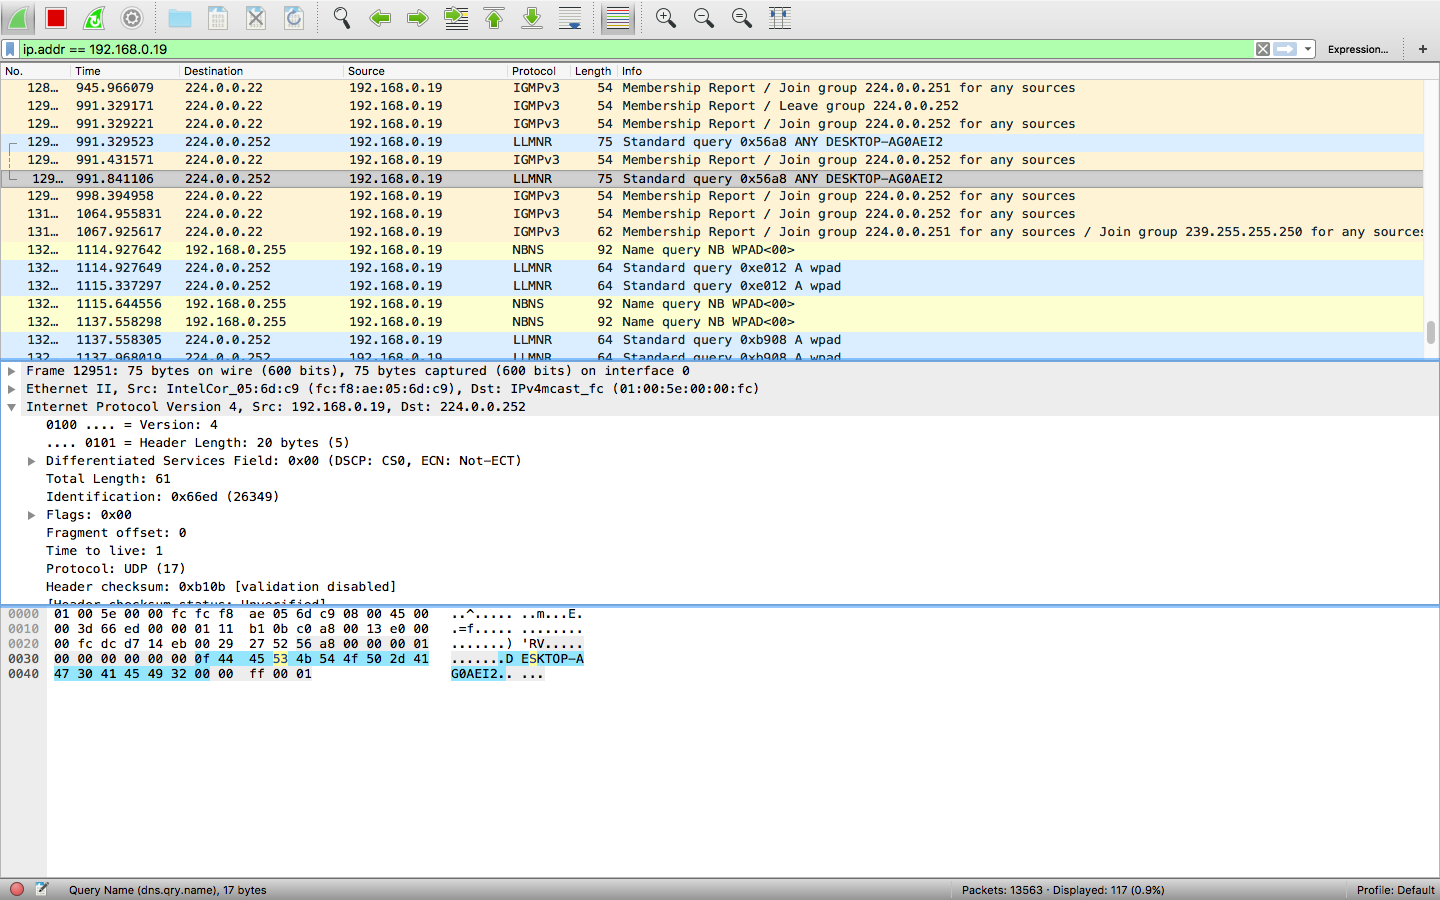
\includegraphics[scale=0.2]{images/wire1.png}
    \caption{Wireshark}
    \label{fig:my_label}
\end{figure}
\newpage
Una de las ventajas de Wireshark es que se puede realizar un análisis de trafico de los equipos conectados a la red, lo que permite que se pueda ver la actividad realizada, vale decir, si un equipo ingresa a una pagina web en especifico este puede ser localizado, por ejemplo y como propuso el ayudante, se ingreso a la pagina de la universidad, obteniéndose lo siguiente:
\begin{figure}[h]
    \centering
    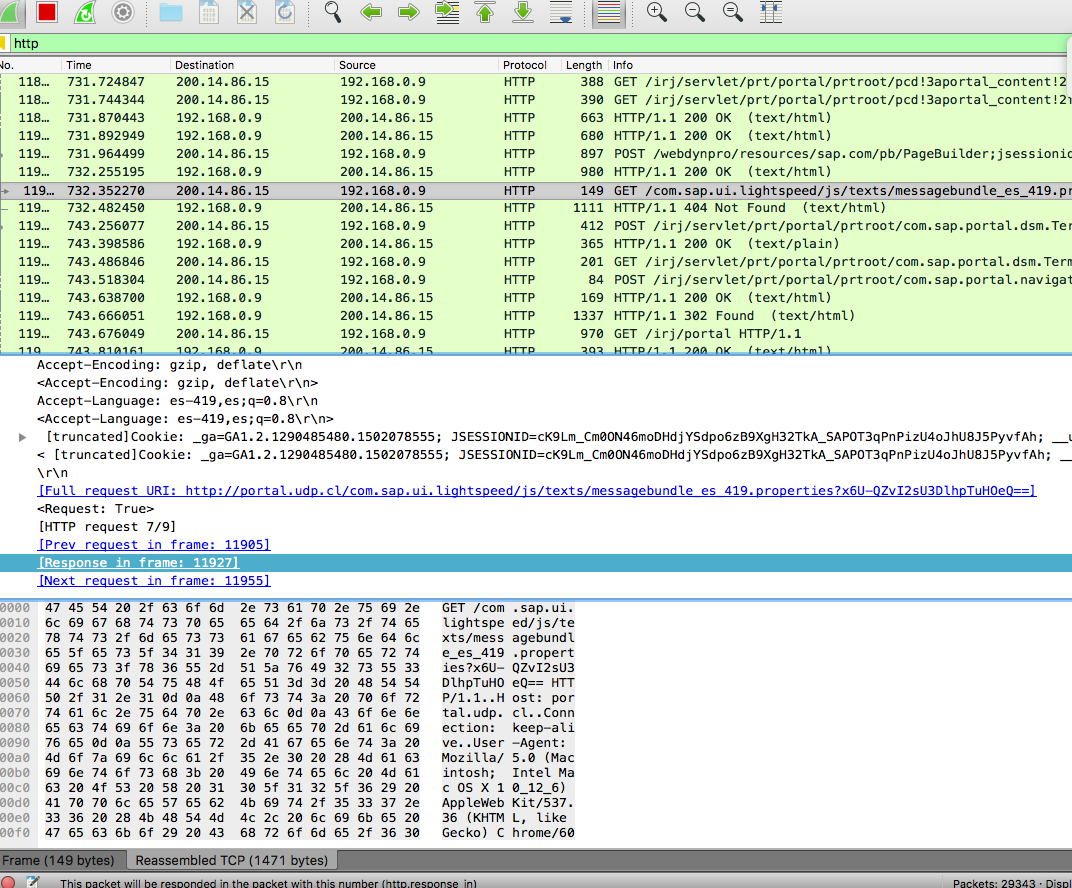
\includegraphics[scale=0.2]{images/wire2.png}
    \caption{Wireshark HTTP}
    \label{fig:my_label}
\end{figure}
\\Como se puede observar de manera a priori se puede ver que dicha IP de origen accedió al sitio de la universidad, hasta el momento no se ha realizado un análisis, es decir, solo se corrobora una parte del potencial de Wireshark.
\section{Creación de paquetes}
Uno de los temas fundamentales de la experiencia de laboratorio fue la creación de paquetes, para ello se utiliza la herramienta llamada Scapy mencionada con anterioridad en los objetivos, para iniciar dicha aplicación, desde la terminal se llama al comando "sudo scapy".
\begin{figure}[h]
    \centering
    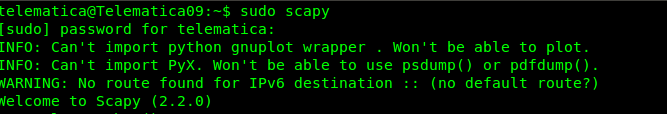
\includegraphics[scale=0.3]{images/in.png}
    \caption{Scapy}
    \label{fig:my_label}
\end{figure}
\\Una vez dentro de Scapy, se procede a crear el paquete, esto implica que se tienen que ir creando capa por capa hasta completarse, a continuación se detallara el proceso de creación de un paquete.
\subsection{Procedimiento}
Uno de los primeros pasos es crear la capa de enlace de la red, para ello se crea una variable que albergue el comando Ether().
\begin{figure}[h]
    \centering
    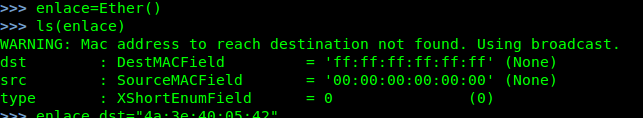
\includegraphics[scale=0.3]{images/enlace.png}
    \caption{Scapy capa enlace}
    \label{fig:my_label}
\end{figure}
\newpage
Observación: Se llama al comando ls(enlace) para mostrar todos los campos de la variable creada. Una vez realizado lo anterior, se observa que en la imagen aparece DST y SRC lo que indican respectivamente, MAC destino y MAC origen, estos se pueden modificar realizando la siguiente operación.
\begin{figure}[h]
    \centering
    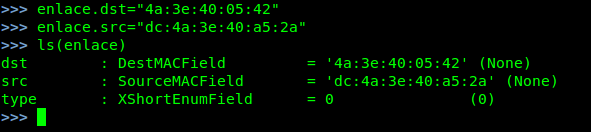
\includegraphics[scale=0.3]{images/1.png}
    \caption{Figura 2}
    \label{fig:my_label}
\end{figure}
\\Cabe mencionar que la MAC de destino no fue al azar ya que se le solicito a un usuario dentro de la red para poder efectuar un envio de paquetes.
\begin{figure}[h]
    \centering
    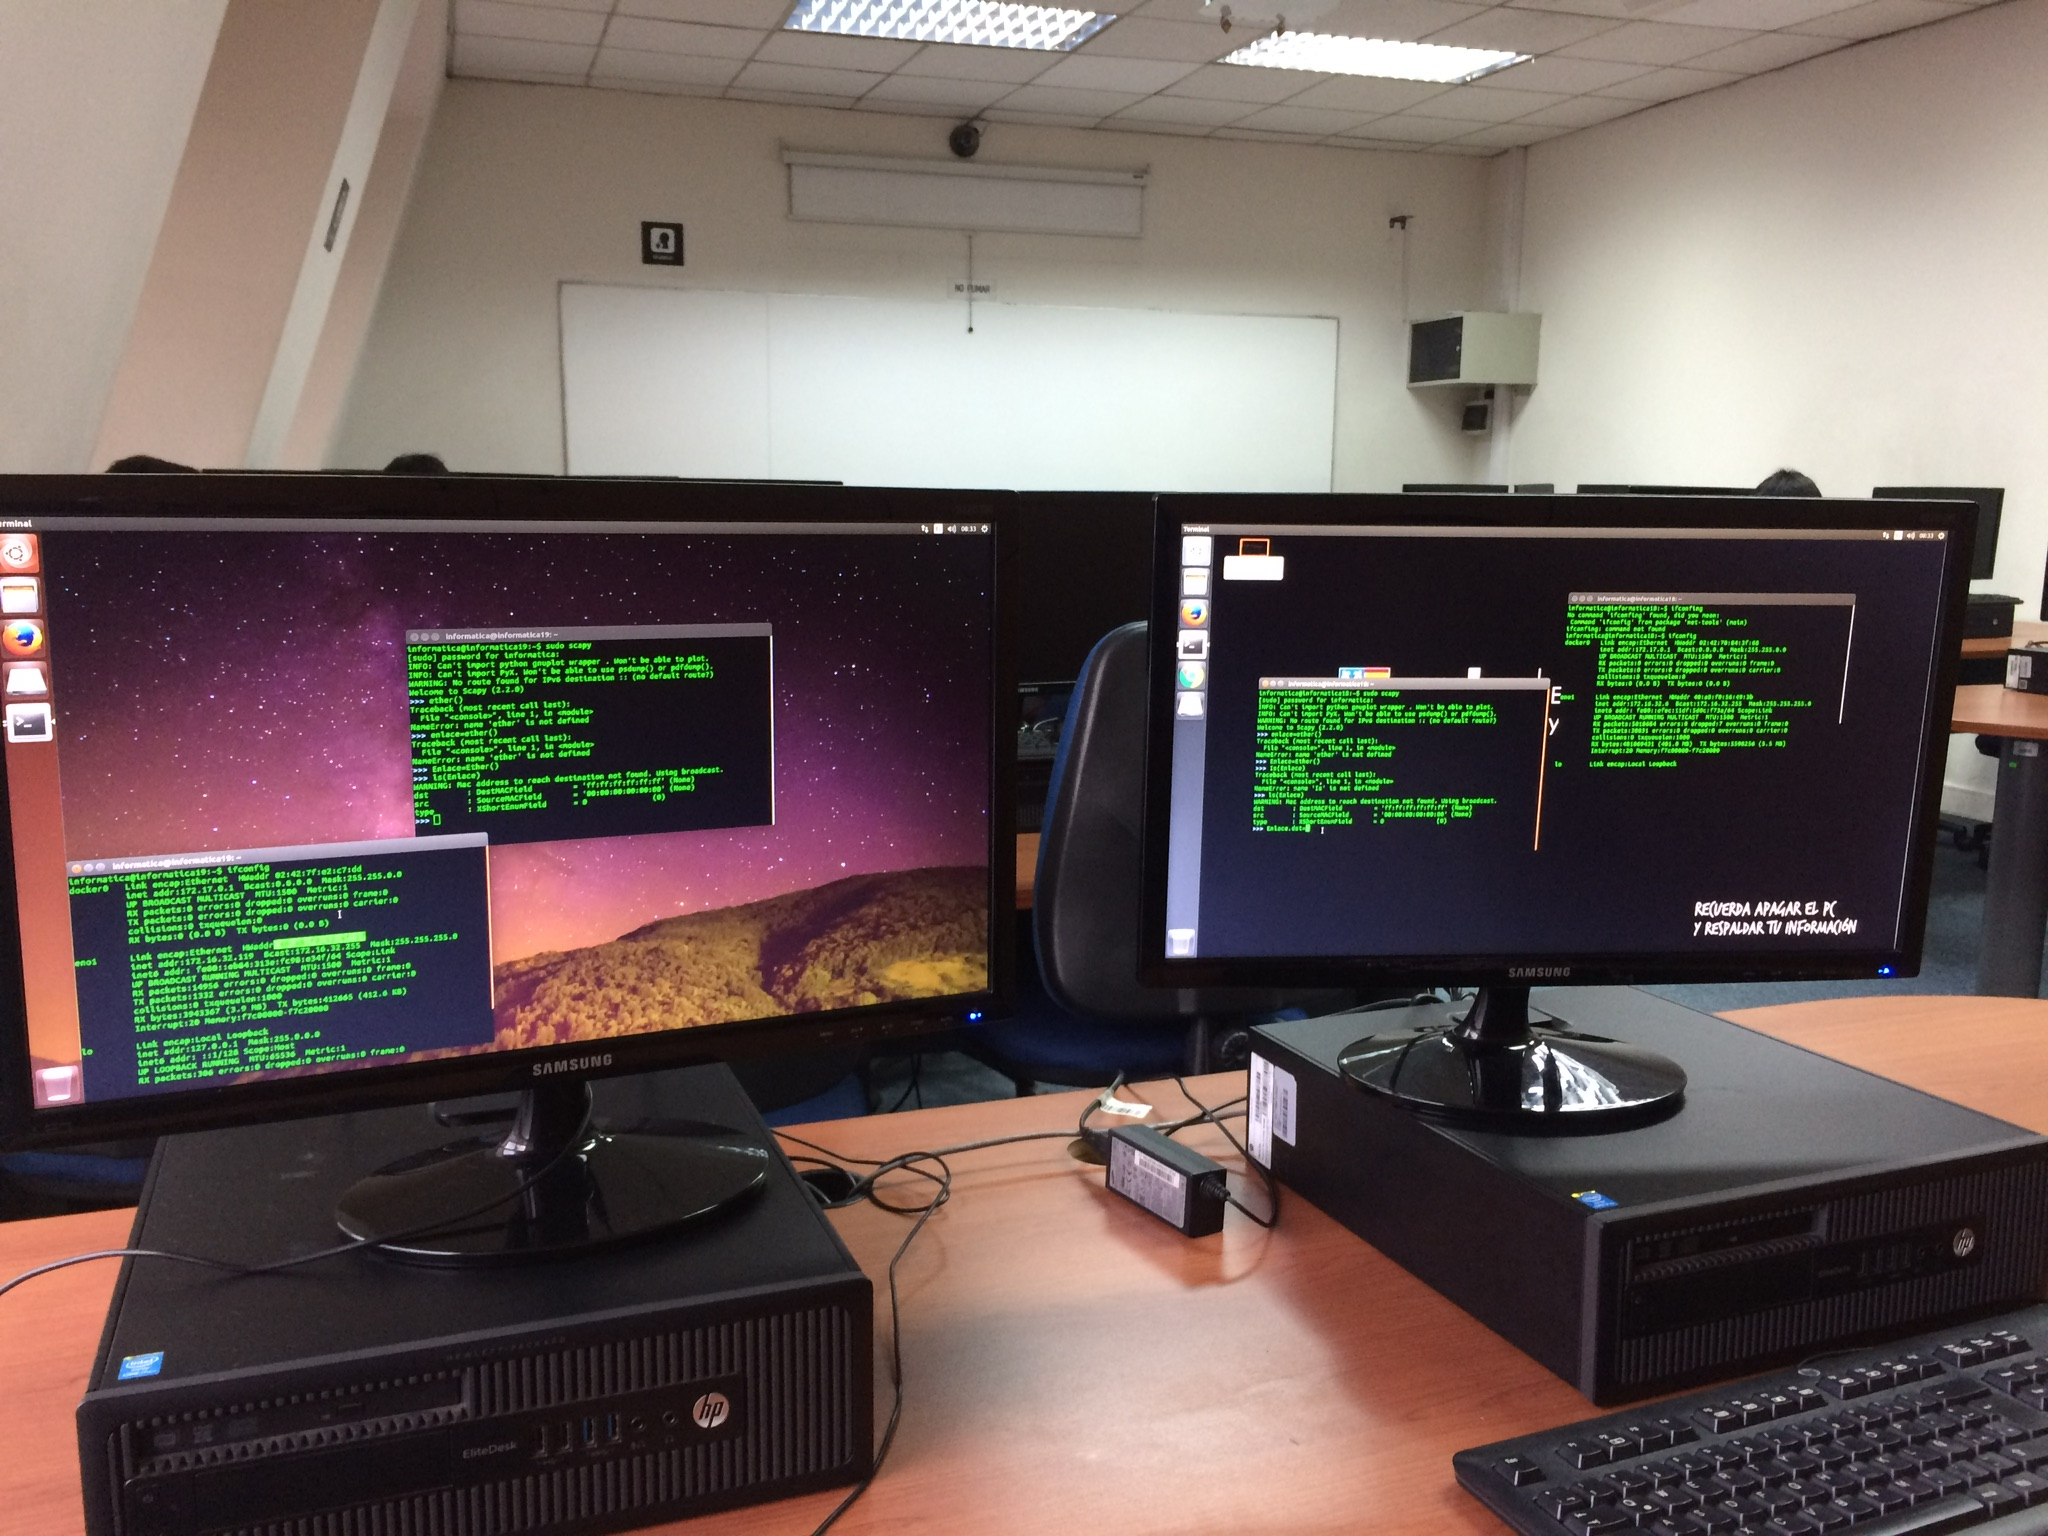
\includegraphics[scale=0.1]{images/2.JPG}
    \caption{Sala}
    \label{fig:my_label}
\end{figure}
\\El paso siguiente es crear la capa de red, al igual que en enlace se crea una variable que almacene el comando IP().
\begin{figure}[h]
    \centering
    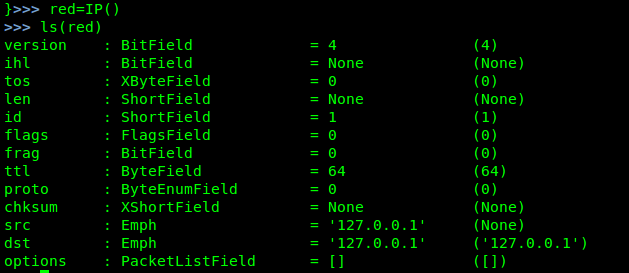
\includegraphics[scale=0.3]{images/2.png}
    \caption{capa red}
    \label{fig:my_label}
\end{figure}
\newpage
Continuando con la capa de transporte, se crea la capa de enlace del paquete, almacenando en otra variable el comando ICMP()
\begin{figure}[h]
    \centering
    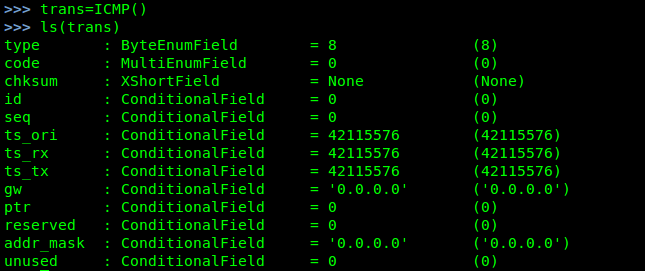
\includegraphics[scale=0.3]{images/3.png}
    \caption{Capa Transporte}
    \label{fig:my_label}
\end{figure}
\\Para finalizar la creación de variables se debe crear una y asignarle el contenido de el comando Raw(), ilustrado a continuación.
\begin{figure}[h]
    \centering
    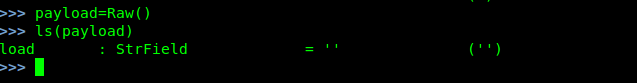
\includegraphics[scale=0.3]{images/4.png}
    \caption{Capa Transporte}
    \label{fig:my_label}
\end{figure}
Una vez creada y asignada todas las capas, es momento de formar el paquete apilando todas las variables asignadas por orden de creación, como se muestra en la imagen...
\begin{figure}[h]
    \centering
    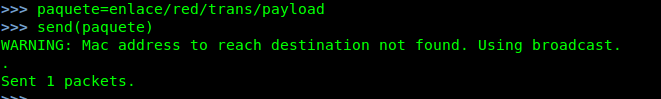
\includegraphics[scale=0.3]{images/5.png}
    \caption{Capa Transporte}
    \label{fig:my_label}
\end{figure}
\subsubsection{Envió de paquete a MAC existente en la red}
Para enviar paquetes con una MAC de destino especifica a través de la red se debe cambiar la dirección de destino en la variable en la que tenemos asignada la capa de enlace, para esto se debe el proceso explicado en el punto 3.2.1 y asignar la MAC del equipo que se desee que llegue el paquete, esto se mostró en la imagen \textbf{Figura 2}\\
\subsubsection{Envio de paquete a MAC inexistente en la red}
En este caso se sigue el mismo proceso que en los casos anteriores solo que esta vez utilizamos una MAC de destino que no existe dentro de la red. luego de enviar el paquete a través de la red aparece un mensaje el cual da una advertencia de que la MAC de destino no existe dentro de la red y que se usara broadcast para enviar el paquete, por lo que este llego a todos los equipos de la red.
\begin{figure}[h]
    \centering
    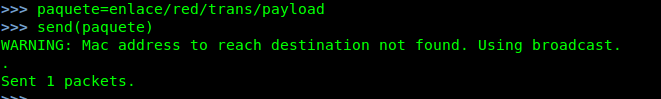
\includegraphics[scale=0.3]{images/5.png}
    \caption{Broadcast}
    \label{fig:my_label}
\end{figure}
\newpage
\section{Visualización En Wireshark}
Luego de  la creación del paquete y paso ultimo de la experiencia de laboratorio, se procede a validar si el paquete realizo alguno de los envíos de paquetes realizados, de lo realizado no se pudo obtener satisfactoriamente la captura del ping, arrojando lo siguiente
\begin{figure}[h]
    \centering
    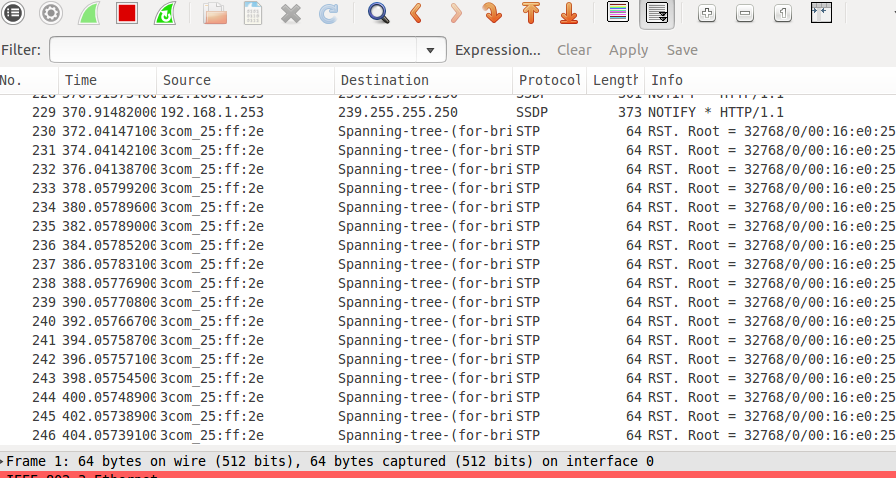
\includegraphics[scale=0.3]{images/6.png}
    \caption{Resultado Wireshark}
    \label{fig:my_label}
\end{figure}
\chapter{Cuestionario}
\begin{enumerate}
    \item ¿Qué sucede cuando envió un paquete a la dirección FF:FF:FF:FF:FF:FF?¿Quiénes lo reciben? ¿Por qué?:
    \\[0.2 cm] El paquete lo reciben todos los que estén conectados al segmento de red en la que actualmente se esta conectado, esto es por que la  la dirección FF:FF:FF:FF:FF:FF se le conoce como dirección de difusión, en otras palabras hace un envio Broadcast del paquete en cuestión, este paquete actúa como una petición para que un nodo con determinada IP responda al llamado otorgando su dirección MAC
    \item ¿Qué pasa cuando envió un paquete con MAC destino a un equipo que no se encuentra en la red? ¿Quiénes lo reciben? ¿Por qué?
    \\[0.2cm] Cuando envió un paquete con una MAC destino la cual no esta en la red de origen, se tendrá que proceder atravesar los routers para ir viendo en otras redes si se encuentra el equipo con la MAC especificada. En otras palabras se tendrá que enviar el paquete al router de la red en la que esta el equipo de origen, para ello se tendrá que formular una petición ARP solicitando su dirección física(la del router) para así crear una puerta de enlace que permitirá al router transferir el mensaje comunicar con otras redes hasta llegar a la MAC destino inicial.
    \item ¿Qué pasa cuando envió un paquete con MAC destino a un equipo de la red? ¿Quiénes lo reciben? ¿Por qué?
    \\[0.2cm]El paquete es recibido por el equipo con la MAC especificada , esto es por que el paquete sera enviado de manera Unicast, al ser de la capa de enlace el Switch sera el encargado de hacer el envio unicamente a ese equipo con la MAC especificada.
    \item ¿Cuál es la diferencia entre una página HTTP y otra HTTPS?
    \\[0.2cm]La diferencia radica en la seguridad de navegación, HTTP es un protocolo orientado a tener un funcionamiento del tipo petición- respuesta, siendo el usuario quien forme la petición y el servidor la respuesta, esto hace que sea muy vulnerable al no tener cifrado. En cuanto a HTTPS realiza su funcionamiento en base a petición-respuesta (similar a HTTP) pero su diferencia es que este es cifrado lo que hace que sea más seguro navegar en este tipo de protocolos.
    \item ¿En que podría influir en una compañía que los datos no sean seguros? Fundamente su respuesta.
    \\[0.2cm]Podría suceder que la información exclusiva de la empresa y sus usuarios salga de esa "esfera" a otros usuarios externos los cuales dependiendo de las intenciones y la importancia de lo que se transmita, puedan ver la información contenida provocando así en caso de querer, la perdida de la información o modificación, inclusive plagiar lo contenido en dicho paquete.

\end{enumerate}
\newpage
\chapter{Conclusión}
De la presente experiencia de laboratorio se concluye inicialmente que fue satisfactoria en términos de conocimientos, si bien la actividad practica se realizado al pie de la letra, no todos los objetivos se pudieron cumplir satisfactoriamente, esto se pudo deber a algún error en la recepción de una dirección MAC de destino o por el mal manejo del programa Wireshark.
\\ Uno de los puntos fuertes de dicha experiencia fue la creación de paquetes usando la herramienta Scapy, comprendiendo la manera adecuada de implementar paquetes. 
\begin{thebibliography}{0}
\bibitem{1}Scapy. Recuperado de https://www.seguridadx.com/scapy/
\bibitem{2}Movimiento de datos en la red. Recuperado de http://ecovi.uagro.mx/ccna1/course/module3/3.3.3.2/3.3.3.2.html
\bibitem{3}Seguridad Informatica. Recuperado de https://definicion.de/seguridad-informatica/
\end{thebibliography}
\listoffigures
\end{document}

